%!TEX root = ./report.tex

\section{Dynamic Programming}
The weights for the tracking and the obstacle avoidance cost are set to the values provided in the code comments.
In particular, the weights are set to
\begin{eqnarray}
	\omega_{track-d} &=& 10\, ,\\
	\omega_{track-heading} &=& 20\, ,\\
	\omega_{collision-avoidance} &=& 100 \, .
\end{eqnarray}
\subsection{Experiments}
Figure~\ref{fig:dyn_prog_results} shows the results for two different paths with obstacle avoidance disable (left) and enabled, respectively.
Obviously, the obstacle avoidance does indeed produce collision free paths with the weights given above.
As the cost decays cubically with the distance to an obstacle the vehicle still might pass close by obstacle, but would not not collide.
For instance, consider the obstacle at $(17, 54)$ in Figure~\ref{fig:dyn_prog_results}~(d).
The visualization is a bit misleading, but in fact the vehicle does not collide, but passes by the obstacle in a distance of approximately $0.5m$.

\begin{figure}[h]
	\begin{subfigure}{.49\textwidth}
		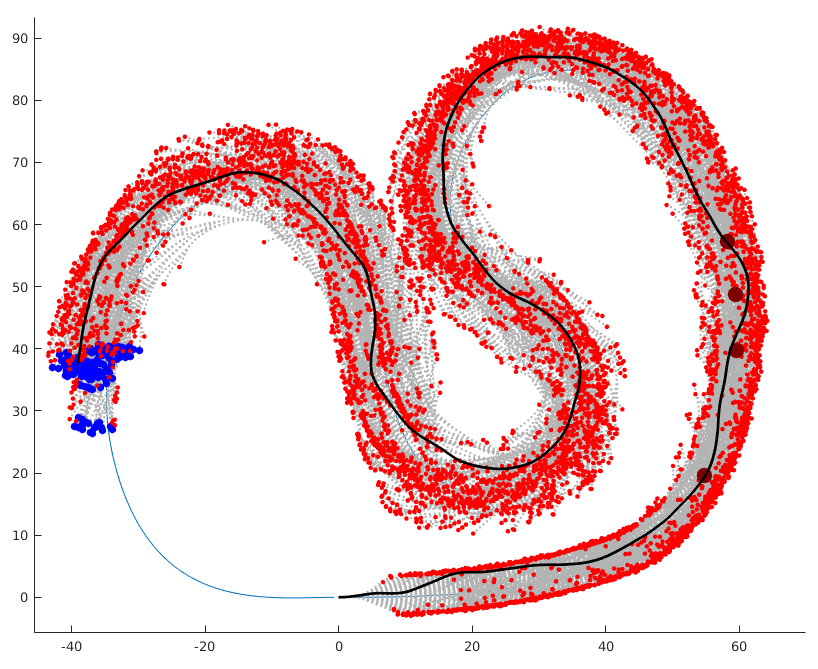
\includegraphics[width=\textwidth]{figures/dyn_prog_no_obs_avoid.png}
		\subcaption{No obstacle avoidance, path 3}
	\end{subfigure}
	\begin{subfigure}{.49\textwidth}
		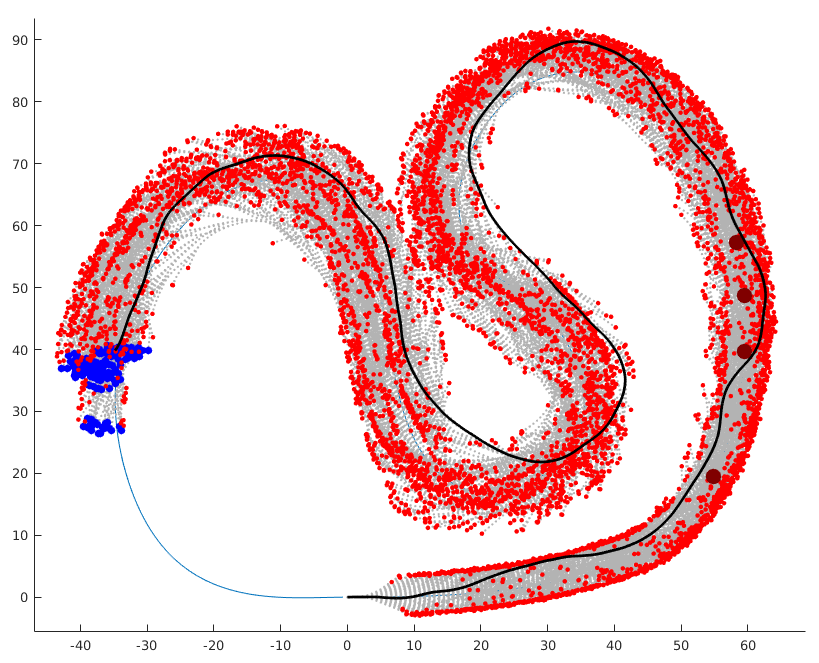
\includegraphics[width=\textwidth]{figures/dyn_prog_obs_avoid.png}
		\subcaption{Obstacle avoidance, path 3}
	\end{subfigure}
	\begin{subfigure}{.49\textwidth}
		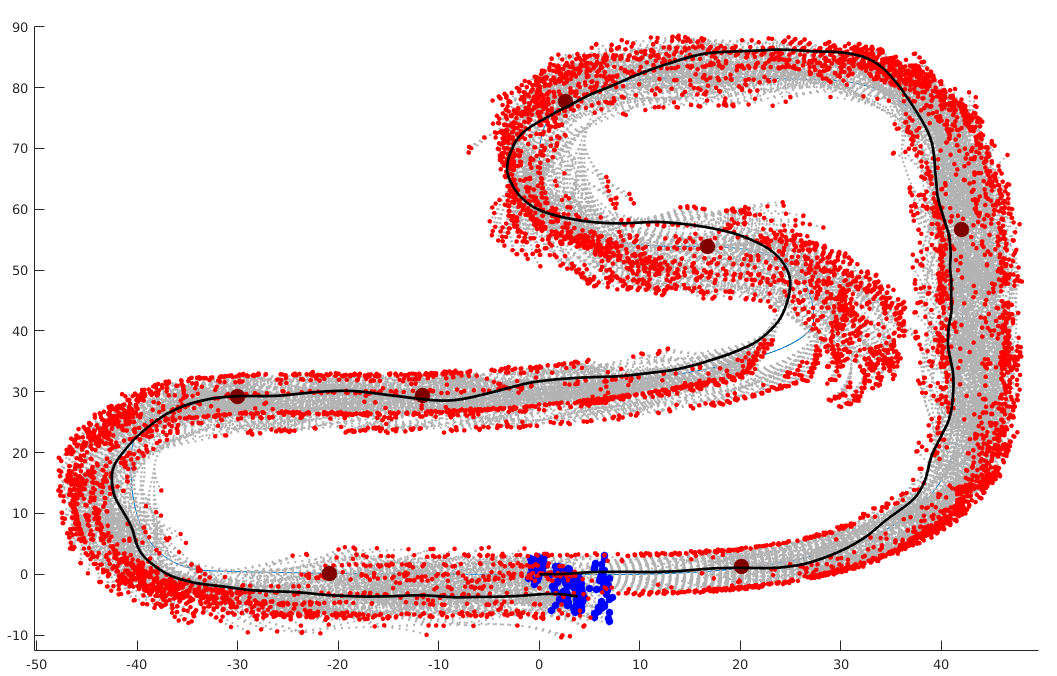
\includegraphics[width=\textwidth]{figures/dyn_prog_no_obs_avoid_2.png}
		\subcaption{No obstacle avoidance, path 2}
	\end{subfigure}
	\begin{subfigure}{.49\textwidth}
		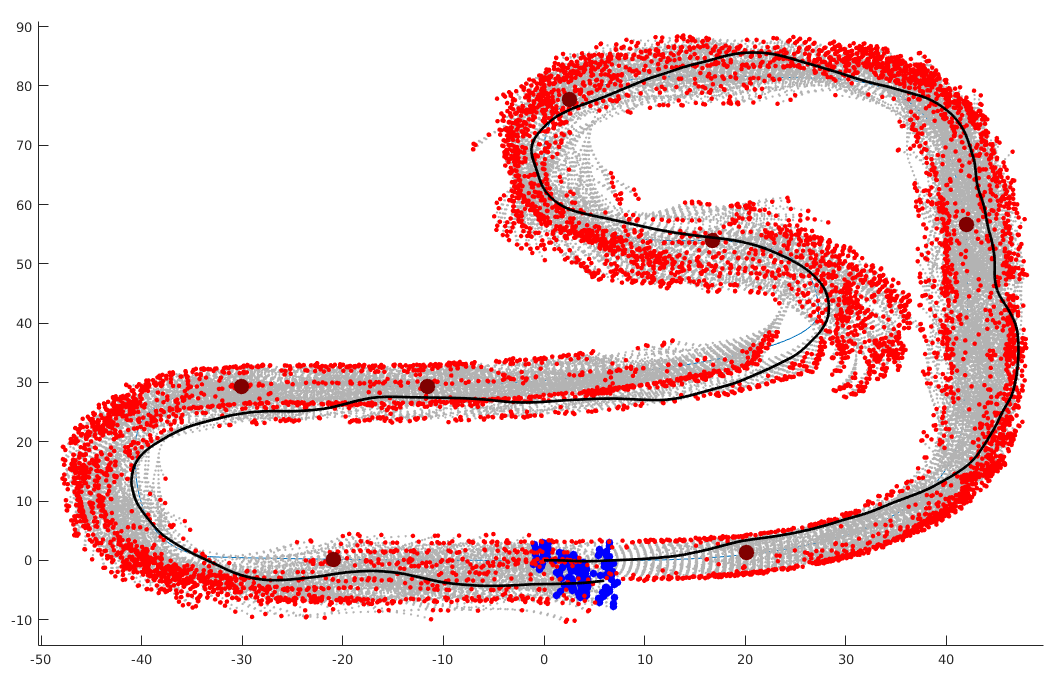
\includegraphics[width=\textwidth]{figures/dyn_prog_obs_avoid_2.png}
		\subcaption{Obstacle avoidance, path 2}
	\end{subfigure}
	\caption{Performance of the dynamic programming approach for path tracking. On the left the obstacle avoid is disables ($\omega_{obs} = 0$) and on the right it is activated with cost $\omega_{obs} = 100$.}
	\label{fig:dyn_prog_results}
\end{figure}

\subsection{Does it Always Find a Collision-free Path?}
\paragraph{Short answer:} No.

\paragraph{Long answer:} First, one needs to define the term \emph{collision free}.
In the setting here, all obstacles are points and are infinitely small.
Therefore, a path is collision free if it will not pass \emph{exactly} through an obstacle in the setting here.
It seems quite hard to pass \emph{exactly} through an obstacle and so it should be easy to find non-colliding trajectories.
However, as shown below it quite easy to construct settings, where no collision-free path can be found.

Note that for a finite amount of nodes in the graph there is only a finite amount of possible control actions, as the control actions to get to the next state are picked from the fixed and finite set of possible control actions $\Omega$.
Therefore, one can easily construct settings where the algorithm can not find a collision-free solution by picking a time $t$ and placing an obstacle at all the places the vehicle can be at that time given the fixed set of control actions $\Omega$.
One such construction is to pick $t=0$ and place an obstacle at the starting position of the vehicle.
Then, every node cost will be infinite and the dynamic programming approach can never find a collision-free path in this case.

\subsection{Why Randomization?}
When the graph is constructed, each control action can be performed at each node.
Let $N(t)$ be the nodes of the graph at time $t$.
As each control actions can be performed at each node the next layer of the graph would in theory have
\begin{equation}
	|N(t+1)| = |N(t)| \cdot |\Omega|
\end{equation}
nodes, where $\Omega$ denotes the set of possible control actions. 
This would lead to an exponentially growing graph with
\begin{equation}
	|N(t)| = |N(0)| \cdot |\Omega|^t\
\end{equation}
nodes after the $t$-th step.
Of course this is infeasible and can not be computed within reasonable time and space complexity.
In order to limit the growth of the graph the number of nodes per layer is limited to an upper bound $n_{max}$.
Then, if at time $t+1$ more than $n_{max}$ nodes are generated, a total number of $n_{max}$ will be randomly picked from the newly generated nodes and the remaining will be discarded.
Using this approach the number of nodes only grows $\mathcal{O}(n_{max}\cdot t)$ and not according to $\mathcal{O}(|\Omega|^t)$ and is therefore linear and not exponential in time.
Further, the nodes must be selected randomly as one would privilege some specific behavior else.

\subsection{Discussion}
The cost-based obstacle avoidance with the cubically decreasing cost for obstacle distance does work to produce collision-free paths, but these paths are sometime weird and do not behave as one would predict in the first place.
It is hard to find a cost setting, where the performance is good for every obstacle.
One such example is shown in Figure~\ref{fig:dyn_prog_discussion}.
A wall of many of the (infinitely small) obstacles with a gap is constructed and horizontally shifted into four different positions.
The columns in the Figure each show one setting of the wall position.
In the top row a low obstacle avoidance cost $\omega_{obs}=10$ is used and in the bottom row a high cost of $\omega_{obs}=1000$.
For the first setting the high cost produces a better result, while for setting 3 the low cost is better.

Further note, that the wall is not symmetric around the gap, i.e. there are more obstacles in the row left of the gap than on the right.
This also affects the trajectory of the vehicle as for example visible in Figure~\ref{fig:dyn_prog_discussion}~(e).
One could argue that this does not really make sense, as a human driver would try to pass in the middle of the gap.

\begin{figure}[h]
	\begin{subfigure}{.24\textwidth}
	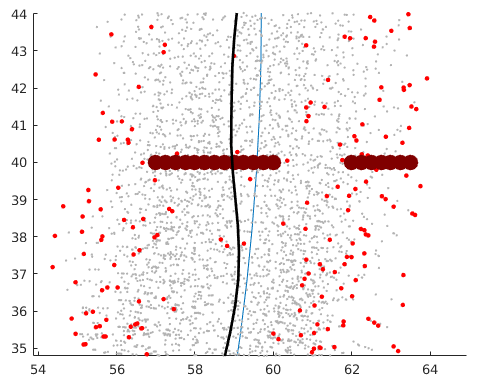
\includegraphics[width=\textwidth]{figures/dyn_prog_dis_1_low.png}
	\subcaption{Setting 1, $\omega_{obs}=10$}
	\end{subfigure}
	\begin{subfigure}{.24\textwidth}
	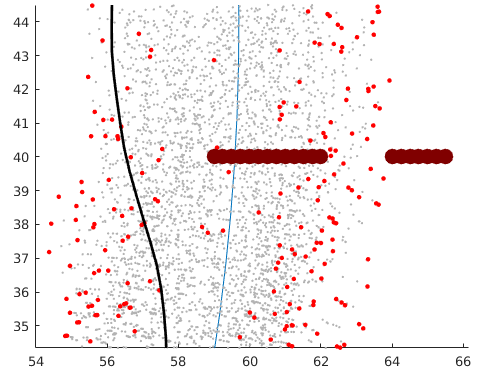
\includegraphics[width=\textwidth]{figures/dyn_prog_dis_2_low.png}
	\subcaption{Setting 2, $\omega_{obs}=10$}
	\end{subfigure}
	\begin{subfigure}{.24\textwidth}
	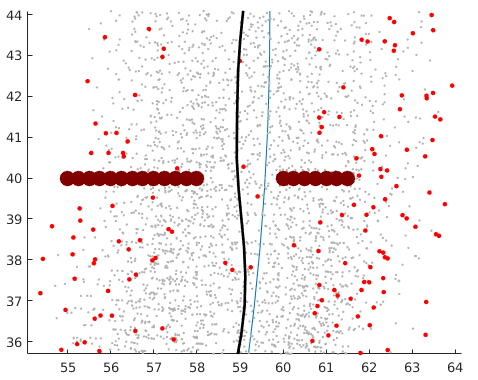
\includegraphics[width=\textwidth]{figures/dyn_prog_dis_3_low.png}
	\subcaption{Setting 3, $\omega_{obs}=10$}
	\end{subfigure}
	\begin{subfigure}{.24\textwidth}
	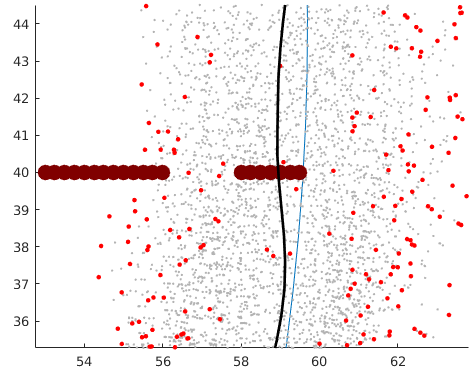
\includegraphics[width=\textwidth]{figures/dyn_prog_dis_4_low.png}
	\subcaption{Setting 4, $\omega_{obs}=10$}
	\end{subfigure}
	\begin{subfigure}{.24\textwidth}
	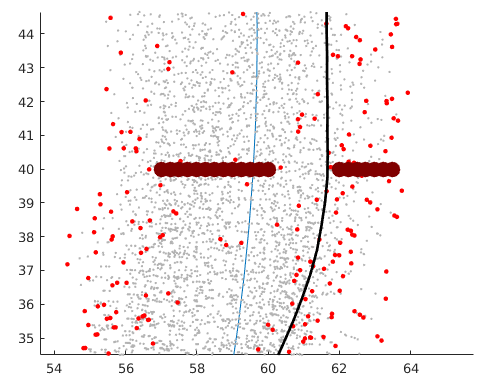
\includegraphics[width=\textwidth]{figures/dyn_prog_dis_1_high.png}
	\subcaption{Setting 1, $\omega_{obs}=1000$}
	\end{subfigure}
	\begin{subfigure}{.24\textwidth}
	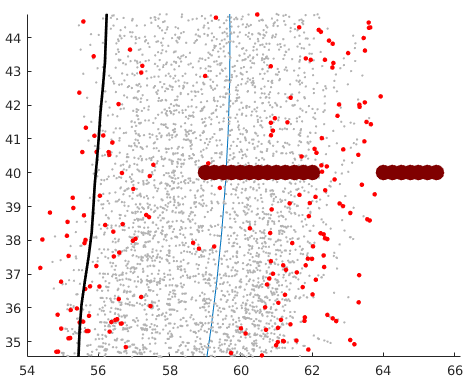
\includegraphics[width=\textwidth]{figures/dyn_prog_dis_2_high.png}
	\subcaption{Setting 2, $\omega_{obs}=1000$}
	\end{subfigure}
	\begin{subfigure}{.24\textwidth}
	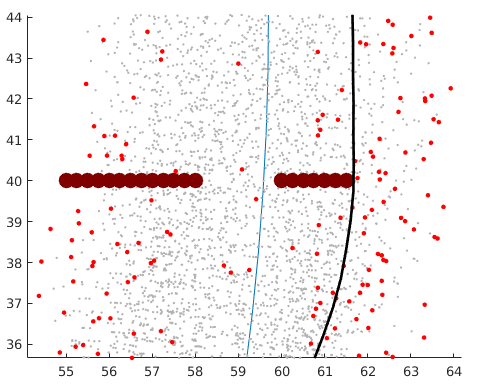
\includegraphics[width=\textwidth]{figures/dyn_prog_dis_3_high.png}
	\subcaption{Setting 3, $\omega_{obs}=1000$}
	\end{subfigure}
	\begin{subfigure}{.24\textwidth}
	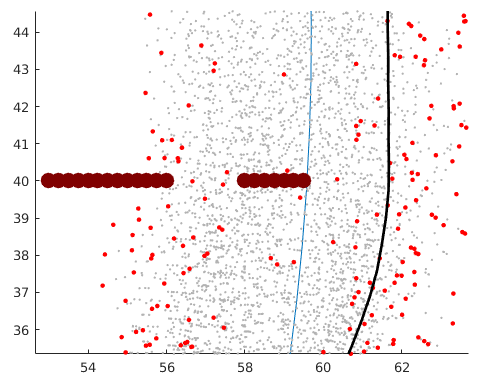
\includegraphics[width=\textwidth]{figures/dyn_prog_dis_4_high.png}
	\subcaption{Setting 4, $\omega_{obs}=1000$}
	\end{subfigure}
	\caption{Four different settings of an obstacle wall for two different obstacle avoidance costs $\omega_{collision-avoidance} = \omega_{obs}$. For some settings the low cost and for some settings the high cost performs better.}
	\label{fig:dyn_prog_discussion}
\end{figure}

